\documentclass[conference]{IEEEtran}

\IEEEoverridecommandlockouts

\usepackage{cite}
\usepackage{amsmath,amssymb}
\usepackage{booktabs}
\usepackage{graphicx}
\usepackage{array}
\usepackage{multirow}
\usepackage{url}
\usepackage{tikz}
\usepackage{xcolor}
\usepackage{listings}
\usepackage{placeins}
\usepackage{balance}

\usetikzlibrary{arrows.meta,positioning,shapes.geometric,shapes.misc,calc}

\definecolor{sfblue}{RGB}{72,91,180}
\definecolor{sfgreen}{RGB}{42,150,88}
\definecolor{sforange}{RGB}{204,116,39}
\definecolor{sfred}{RGB}{185,55,55}
\definecolor{sflight}{RGB}{244,246,255}

\lstdefinestyle{codeblock}{
  basicstyle=\ttfamily\footnotesize,
  breaklines=true,
  frame=single,
  columns=fullflexible,
  showstringspaces=false,
  tabsize=2
}

\setlength{\textfloatsep}{8pt plus 2pt minus 2pt}
\setlength{\floatsep}{7pt plus 2pt minus 2pt}
\setlength{\intextsep}{7pt plus 2pt minus 2pt}

\title{SmartFocus: An Attention-Aware Gamified Adaptive Learning System Using Computer Vision and Knowledge Graphs}

\author{
\IEEEauthorblockN{Shankar Patel K. U.}
\IEEEauthorblockA{\textit{Department of Information Science Engineering}\\
R. V. College of Engineering\\
Bengaluru, India\\
1RV23IS109}
\and
\IEEEauthorblockN{Spandana K. N.}
\IEEEauthorblockA{\textit{Department of Information Science Engineering}\\
R. V. College of Engineering\\
Bengaluru, India\\
1RV23IS115}
\and
\IEEEauthorblockN{Mainak Sen}
\IEEEauthorblockA{\textit{Department of Industrial Engineering and Management}\\
R. V. College of Engineering\\
Bengaluru, India\\
1RV23IM029}
}

\begin{document}

\maketitle

\begin{abstract}
Online learning systems usually know whether a student answered a question correctly, but they rarely know whether the student was attentive, tired, or bored while answering it. This missing context often leads to rigid learning paths: a sleepy learner may still receive difficult questions, while a learner who has already understood a topic may be forced through repeated easy material. SmartFocus was built to reduce this gap. It is a browser-based adaptive learning platform that combines webcam-based attention estimation, a prerequisite knowledge graph, and game-like progression. The browser captures webcam frames and streams them to a FastAPI backend through WebSocket. A computer vision pipeline based on OpenCV face and eye detection and facial emotion classification estimates a focus score and maps the learner state into three practical labels: FOCUSED, BORED, and SLEEPY. These live signals are combined with answer correctness, response time, question difficulty, and concept mastery to choose the next question from a Python programming question bank. The learning domain is represented as a directed graph of 33 Python concepts with prerequisite links, allowing the system to recommend unlocked topics and identify bottleneck concepts. A React frontend presents this adaptation through quests, a skill tree, XP, badges, and boss battles, while a teacher dashboard summarizes focus trends and student risk. Prototype testing reported 84\% three-class emotion recognition accuracy, 91\% face detection rate, and a clear shift from easy to hard questions as mastery increased.
\end{abstract}

\begin{IEEEkeywords}
adaptive learning, affective computing, computer vision, gamification, knowledge graph, OpenCV, Neo4j, WebSocket, Bloom's taxonomy
\end{IEEEkeywords}

\section{Introduction}

Digital learning platforms have become a normal part of academic life, especially for programming and technical subjects. Earlier work on adaptive hypermedia and intelligent tutoring systems shows that learner models can improve personalization when the system tracks progress over time \cite{brusilovsky1996methods,vanlehn2005andes,corbett1994knowledge}. Their reach is high, but their ability to react like a human tutor is still limited. In a classroom, a teacher can notice that a student is losing attention, slowing down, or becoming bored. The teacher may pause, repeat a concept, give a hint, or increase the challenge. Many online systems, in contrast, make decisions mostly from answer history. They know what was clicked, but not the condition under which the click happened.

This is a serious limitation in programming education. Concepts in Python are not isolated. Variables and data types support operators; operators support conditionals; conditionals support loops and functions; later topics such as recursion, decorators, and object-oriented programming depend on several earlier ideas. Work on knowledge tracing and prerequisite relations also supports the idea that learning systems should reason about concept dependencies, not only final marks \cite{corbett1994knowledge,pan2017prerequisite}. A student who is pushed forward without prerequisite mastery can struggle quickly. At the same time, a student who is attentive and already performing well may lose interest if the platform continues to ask simple questions.

SmartFocus is designed around the view that adaptation should consider both knowledge state and attention state. This view is influenced by affective computing, where emotional and attentional cues are treated as meaningful signals during interaction \cite{picard1997affective,dmello2012dynamics}. The platform uses a webcam-based computer vision pipeline to estimate whether a learner is focused, bored, or sleepy. The same session records answer correctness, response time, and question difficulty. These signals are fed into a graph-based adaptive engine that recommends questions and concepts from a prerequisite map of Python programming topics. The student experiences this as an interactive learning game: quests, XP, a skill tree, badges, and boss battles. The teacher sees focus history, risk levels, and concepts that block class progress.

\section{Problem Statement and Objectives}

Most online learning tools adapt only after a student submits an answer. This creates a delay between the learner's real condition and the system response. A student may be tired, distracted, or bored, but the platform still asks the same style of question because it has no live attention signal. The problem becomes sharper in programming courses because concepts are strongly connected. If an early prerequisite is weak, later topics become difficult even when the student keeps attempting questions.

The problem addressed in this project is to design a learning system that can observe attention during practice, combine that signal with concept mastery, and select the next learning activity in a way that feels natural to the learner.

The objectives of SmartFocus are:
\begin{itemize}
  \item to estimate learner attention and emotion from webcam frames in real time;
  \item to maintain a prerequisite graph for Python programming concepts;
  \item to update concept mastery using correctness, focus, emotion, response time, and difficulty;
  \item to present progress through quests, XP, skill-tree states, badges, and boss battles;
  \item to provide teachers with focus trends, risk indicators, and bottleneck concepts.
\end{itemize}

The scope of the prototype is limited to Python programming practice, a browser-based student interface, teacher analytics, and a backend that can run with Neo4j or a local NetworkX graph fallback.

\section{Related Work}

Adaptive learning systems have been studied for several decades. Early adaptive hypermedia systems personalized content according to user models and navigation history \cite{brusilovsky1996methods}. Intelligent tutoring systems such as Andes showed that step-level feedback and learner modeling can improve learning in structured domains \cite{vanlehn2005andes}. Knowledge tracing models estimate how student knowledge changes as attempts are made over time \cite{corbett1994knowledge}. Item Response Theory has also been used to estimate learner ability and match question difficulty to performance \cite{lord1980irt}. These methods are valuable, but many of them focus mainly on correctness and item difficulty.

Affective computing introduced the idea that software can detect and respond to human emotional states \cite{picard1997affective}. In learning, emotions such as boredom, confusion, and frustration are not side details; they influence persistence and performance \cite{dmello2012dynamics}. Prior work has explored facial cues for recognizing frustration and other learning-related states \cite{grafsgaard2013recognizing}. Facial-expression recognition research has also been supported by benchmark datasets and challenges such as FER-2013 and AffectNet \cite{goodfellow2013challenges,mollahosseini2017affectnet}. These works make webcam-based learning state estimation more practical, although classroom lighting, pose, and camera quality remain difficult.

Knowledge graphs provide a natural representation for educational domains where prerequisite relations matter. A graph can store that one concept must be understood before another, and traversal algorithms can identify unlocked topics or weak prerequisites \cite{pan2017prerequisite}. Graph databases are useful when relationships are central to the query, while in-memory graph libraries allow similar logic to run offline during development and testing.

Gamification adds points, badges, levels, challenges, and feedback loops to non-game tasks \cite{deterding2011gamification}. In education, these elements can increase participation when they support learning rather than distract from it \cite{hamari2014gamification}. Motivation research also suggests that challenge, feedback, and a visible sense of competence can support learner engagement when used carefully \cite{ryan2000self}. SmartFocus combines these lines of work. It uses affective signals to decide how difficult the next step should be, a concept graph to decide what can be learned next, and gamification to make progress concrete.

The question bank uses Bloom-style cognitive levels to organize questions from simpler recall to deeper application and analysis. Bloom's taxonomy and its later revision are widely used for structuring learning outcomes \cite{bloom1956taxonomy,anderson2001taxonomy}. Cognitive load theory also supports the need to avoid overwhelming learners when task difficulty rises faster than understanding \cite{sweller1988cognitive}.

\section{Proposed Methodology and System Architecture}

SmartFocus follows a three-tier architecture, shown in Fig.~\ref{fig:architecture}. The frontend is a React and TypeScript application. It handles authentication screens, dashboard widgets, webcam capture, quest interaction, skill tree rendering, boss battles, and teacher views. The backend is a FastAPI application. It exposes REST endpoints for authentication, quests, graph recommendations, focus history, emotion history, boss battles, and teacher analytics. A WebSocket endpoint handles continuous frame streaming from the browser.

\begin{figure}[!htbp]
  \centering
  \resizebox{\columnwidth}{!}{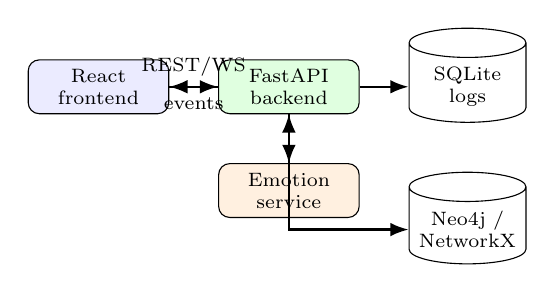
\begin{tikzpicture}[
  font=\scriptsize,
  node distance=0.62cm and 0.62cm,
  box/.style={draw, rounded corners, text width=1.55cm, minimum height=0.52cm, align=center, fill=sflight},
  db/.style={draw, cylinder, shape border rotate=90, aspect=0.25, text width=1.25cm, minimum height=0.52cm, align=center, fill=white},
  arrow/.style={-Latex, thick}
]

\node[box, fill=blue!8] (browser) {React\\frontend};
\node[box, fill=green!12, right=of browser] (api) {FastAPI\\backend};
\node[db, right=of api] (sqlite) {SQLite\\logs};
\node[db, below=of sqlite] (graph) {Neo4j /\\NetworkX};
\node[box, below=of api, fill=orange!12] (emotion) {Emotion\\service};

\draw[arrow] (browser) -- node[above]{REST/WS} (api);
\draw[arrow] (api) -- node[below]{events} (browser);
\draw[arrow] (api) -- (sqlite);
\draw[arrow] (api) |- (graph);
\draw[arrow] (api) -- (emotion);
\draw[arrow] (emotion) -- (api);

\end{tikzpicture}
}
  \caption{Three-tier architecture used in SmartFocus. REST calls handle learning data, while WebSocket carries the live vision stream.}
  \label{fig:architecture}
\end{figure}

SQLite is used for users, sessions, focus logs, emotion logs, quest progress, and boss battle state. The learning graph can run in two modes. In live mode, Neo4j stores concepts and student mastery relations. In mock mode, NetworkX provides an in-memory directed graph. This second mode is useful for demonstrations and development because the platform remains functional even without a graph database connection.

The student workflow begins with login and webcam permission. A hidden monitor component captures frames from the shared camera stream and sends them to the backend. The backend responds with focus, emotion, and bounding-box updates. When the student starts a quest or concept practice session, the adaptive engine selects a question using the current graph mastery and live attention state. After each answer, mastery and XP are updated. If the learner appears sleepy or repeatedly answers incorrectly, the next question becomes easier. If the learner is bored but still focused, the system can move toward harder questions.

\begin{figure}[!htbp]
  \centering
  \resizebox{\columnwidth}{!}{\begin{tikzpicture}[
  font=\scriptsize,
  node distance=0.5cm and 0.45cm,
  step/.style={draw, rounded corners, text width=1.5cm, minimum height=0.5cm, align=center, fill=sflight},
  game/.style={draw, rounded corners, text width=1.5cm, minimum height=0.5cm, align=center, fill=green!10},
  arrow/.style={-Latex, thick}
]

\node[step] (login) {Login};
\node[step, right=of login] (camera) {Camera\\stream};
\node[step, right=of camera] (cv) {Focus +\\emotion};
\node[step, right=of cv] (state) {Learner\\state};

\node[game, below=0.65cm of camera] (quest) {Quest\\question};
\node[game, right=of quest] (answer) {Answer\\submit};
\node[game, right=of answer] (mastery) {Mastery\\+ XP};
\node[game, right=of mastery] (next) {Next\\activity};

\draw[arrow] (login) -- (camera);
\draw[arrow] (camera) -- (cv);
\draw[arrow] (cv) -- (state);
\draw[arrow] (state) |- (quest);
\draw[arrow] (quest) -- (answer);
\draw[arrow] (answer) -- (mastery);
\draw[arrow] (mastery) -- (next);
\draw[arrow] (next.east) -- ++(0.35,0) |- (camera.east);

\end{tikzpicture}
}
  \caption{Student-side learning loop from webcam sensing to mastery update.}
  \label{fig:studentflow}
\end{figure}

\FloatBarrier

\section{Attention and Emotion Estimation}

\subsection{Frame Processing}

The browser captures webcam frames, draws them to a canvas, compresses them as JPEG, and sends the base64 payload to the backend. The backend decodes the bytes into an OpenCV BGR array. The detector first converts the image to grayscale and applies histogram equalization. It then tries multiple Haar cascade detectors, including frontal and profile face cascades. This detector family follows the boosted cascade approach introduced by Viola and Jones \cite{viola2001rapid}. When a face is found, the largest detected face is selected. Eye detection is restricted to the upper portion of the face region because that reduces false detections from the mouth and chin.

The computer vision flow is summarized in Fig.~\ref{fig:cv}. The design intentionally uses a fallback path. If remote emotion inference is unavailable, local FER-style fallback logic or heuristic attention rules still allow the system to produce a usable learning state. This matters for classroom demonstrations and low-connectivity settings.

\begin{figure}[!htbp]
  \centering
  \resizebox{\columnwidth}{!}{\begin{tikzpicture}[
  font=\scriptsize,
  node distance=0.5cm and 0.42cm,
  step/.style={draw, rounded corners, text width=1.42cm, minimum height=0.48cm, align=center, fill=sflight},
  out/.style={draw, rounded corners, text width=1.45cm, minimum height=0.48cm, align=center, fill=green!10},
  arrow/.style={-Latex, thick}
]

\node[step] (frame) {Webcam\\frame};
\node[step, right=of frame] (decode) {Decode\\JPEG};
\node[step, right=of decode] (prep) {Gray +\\equalize};
\node[step, right=of prep] (face) {Face\\cascade};

\node[step, below=0.62cm of decode] (eyes) {Eye ROI\\check};
\node[step, right=of eyes] (emotion) {Emotion\\classifier};
\node[step, right=of emotion] (score) {Focus\\score};
\node[out, right=of score] (event) {WS\\update};

\draw[arrow] (frame) -- (decode);
\draw[arrow] (decode) -- (prep);
\draw[arrow] (prep) -- (face);
\draw[arrow] (face) |- (eyes);
\draw[arrow] (face) |- (emotion);
\draw[arrow] (eyes) -- (emotion);
\draw[arrow] (emotion) -- (score);
\draw[arrow] (score) -- (event);

\end{tikzpicture}
}
  \caption{Computer vision pipeline for attention and emotion estimation.}
  \label{fig:cv}
\end{figure}

\subsection{Focus Score}

The focus score is computed on a 0 to 100 scale. The scoring logic uses three visible signals: whether a face is present, whether the head is centered, and whether eyes appear open. An emotion-based modifier is then applied. The simplified focus formula is:

\begin{equation}
F = 100(0.4P_f + 0.3H_c + 0.3E_o) + M_e
\end{equation}

where \(P_f\) is face presence, \(H_c\) is head centering, \(E_o\) is eye engagement, and \(M_e\) is the emotion modifier. A focused state adds a positive modifier, boredom reduces the score, and sleepiness reduces it more strongly. The WebSocket handler smooths the score using an exponential moving average so that a single noisy frame does not cause sudden user interface changes.

\subsection{Learning State}

The system reduces the vision output into practical learning states. If the learner is focused and the score is high, the state becomes FLOW. If the score is moderate, the state is PRODUCTIVE. Lower scores become STRUGGLING or FATIGUED. A bored expression with low engagement can become DISENGAGED. These states are used in the dashboard, suggestions widget, quest adaptation, and boss battle logic.

\begin{table}[!htbp]
\caption{Live Adaptation Rules Used by the Prototype}
\label{tab:rules}
\centering
\scriptsize
\renewcommand{\arraystretch}{1.12}
\begin{tabular}{p{0.31\linewidth}p{0.47\linewidth}p{0.13\linewidth}}
\toprule
\textbf{Action} & \textbf{Trigger} & \textbf{Cooldown} \\
\midrule
Force break & Focus score below 15 & 120 s \\
Wake prompt & Emotion classified as SLEEPY & 90 s \\
Encouragement & Focus score above 80 & 180 s \\
Increase difficulty & BORED state with high focus & 120 s \\
Reduce difficulty & Low focus or repeated wrong answers & Session rule \\
\bottomrule
\end{tabular}
\end{table}


\FloatBarrier

\section{Graph-Based Adaptive Learning}

\subsection{Concept Graph}

The learning content focuses on Python programming. The graph contains 33 concepts arranged by tier and difficulty, including data types, variables, operators, input-output, conditionals, loops, functions, exception handling, lists, dictionaries, generators, object-oriented programming, inheritance, polymorphism, and decorators. A directed edge represents a prerequisite relation. For example, loops and functions depend on earlier control-flow concepts, while advanced topics depend on several intermediate topics.

For each concept, the graph stores a difficulty level, Bloom level, tier, XP reward, and description. The graph is used to decide which concepts are available, which concepts are still locked, and which concept should be recommended next. A concept is considered mastered when the learner's mastery score crosses the threshold used by the graph engine.

\begin{figure}[!htbp]
  \centering
  \resizebox{\columnwidth}{!}{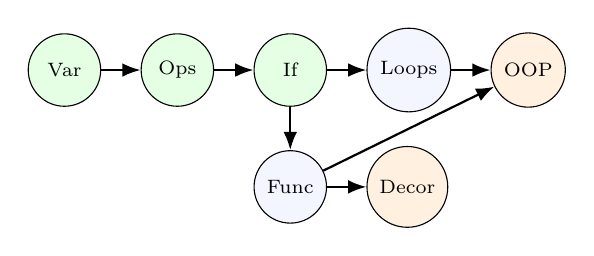
\begin{tikzpicture}[
  font=\scriptsize,
  node distance=0.55cm and 0.5cm,
  concept/.style={draw, circle, minimum size=0.92cm, align=center, fill=sflight},
  core/.style={draw, circle, minimum size=0.92cm, align=center, fill=green!10},
  advanced/.style={draw, circle, minimum size=0.92cm, align=center, fill=orange!12},
  arrow/.style={-Latex, thick}
]

\node[core] (var) {Var};
\node[core, right=of var] (op) {Ops};
\node[core, right=of op] (cond) {If};
\node[concept, right=of cond] (loop) {Loops};
\node[concept, below=0.55cm of cond] (func) {Func};
\node[advanced, right=of loop] (oop) {OOP};
\node[advanced, right=of func] (decor) {Decor};

\draw[arrow] (var) -- (op);
\draw[arrow] (op) -- (cond);
\draw[arrow] (cond) -- (loop);
\draw[arrow] (cond) -- (func);
\draw[arrow] (loop) -- (oop);
\draw[arrow] (func) -- (oop);
\draw[arrow] (func) -- (decor);

\end{tikzpicture}
}
  \caption{Sample prerequisite chain from the Python concept graph.}
  \label{fig:conceptgraph}
\end{figure}

\subsection{Question Bank}

The question bank contains 330 multiple-choice questions across the 33 concepts. Each question has a concept name, difficulty, Bloom level, four options, correct answer, and explanation. Bloom levels follow the revised taxonomy style of arranging questions by cognitive demand \cite{anderson2001taxonomy}. This allows the question selector to choose not only by concept but also by cognitive level.

\subsection{Question Selection}

When a practice session begins, the adaptive engine reads the student's mastery map and selects a concept from the unlocked frontier. It then chooses a question whose difficulty and Bloom level match the learner's current state. Low mastery usually maps to easy questions; growing mastery moves the learner toward medium and hard questions. Attention signals can override this direction. If the learner is sleepy or has very low focus, easier questions are preferred. If the learner is bored while maintaining high focus, the engine increases challenge.

The scoring idea is:

\begin{equation}
S_q = 0.6D_q + 0.3B_q + 0.1R_q
\end{equation}

where \(D_q\) is difficulty alignment, \(B_q\) is Bloom-level alignment, and \(R_q\) is a small random term to reduce repetitive selection. The flow is shown in Fig.~\ref{fig:adaptive}.

\begin{figure}[!htbp]
  \centering
  \resizebox{\columnwidth}{!}{\begin{tikzpicture}[
  font=\scriptsize,
  node distance=0.5cm and 0.42cm,
  step/.style={draw, rounded corners, text width=1.45cm, minimum height=0.5cm, align=center, fill=green!8},
  decision/.style={draw, rounded corners, text width=1.45cm, minimum height=0.5cm, align=center, fill=yellow!18},
  arrow/.style={-Latex, thick}
]

\node[step] (mastery) {Mastery\\map};
\node[step, right=of mastery] (candidates) {Unlocked\\concepts};
\node[decision, right=of candidates] (state) {Focus +\\emotion};
\node[step, right=of state] (target) {Target\\difficulty};

\node[step, below=0.65cm of candidates] (score) {Rank\\questions};
\node[step, right=of score] (select) {Select\\best item};
\node[step, right=of select] (answer) {Record\\answer};
\node[step, right=of answer] (update) {Update\\mastery};

\draw[arrow] (mastery) -- (candidates);
\draw[arrow] (candidates) -- (state);
\draw[arrow] (state) -- (target);
\draw[arrow] (target) |- (score);
\draw[arrow] (score) -- (select);
\draw[arrow] (select) -- (answer);
\draw[arrow] (answer) -- (update);
\draw[arrow] (update.east) -- ++(0.32,0) |- (mastery.east);

\end{tikzpicture}
}
  \caption{Adaptive question selection and mastery update flow.}
  \label{fig:adaptive}
\end{figure}

\FloatBarrier

\subsection{Mastery Update}

After each answer, concept mastery is updated using correctness, difficulty, focus, emotion, and response time. The update is based on a weighted moving estimate:

\begin{equation}
M_{new} = clip(M_{old} + \alpha W_d W_f W_s W_e \Delta, 0, 1)
\end{equation}

Here, \(M_{old}\) is previous mastery, \(M_{new}\) is updated mastery, \(\alpha\) is the base learning rate, \(W_d\) is the difficulty weight, \(W_f\) is the focus weight, \(W_s\) is the speed weight, \(W_e\) is the emotion weight, and \(\Delta\) represents the answer result. Correct answers move mastery upward, while incorrect answers reduce it softly. The weighting means that a fast, correct answer during high focus is treated as stronger evidence of understanding than a slow answer during poor focus.

\section{Gamified Interface}

The student interface presents adaptation through game elements rather than through raw algorithmic messages. The dashboard shows live focus score, emotion state, XP, streak, active quests, and suggestions. The quest board offers concept-linked question sessions with XP rewards. The skill tree visualizes locked, available, and mastered concepts. The boss battle mode converts correct answers into damage and uses focus as a multiplier, making attention visible inside the game mechanics.

Gamification is not used only as decoration. It gives the learner an immediate reason to stay engaged. Combo counters reward answer streaks. Hints reduce the XP multiplier, encouraging students to try independently while still making help available. Boss battles unlock only after sufficient concept progress, turning mastery into a milestone rather than a hidden number.

The teacher dashboard gives an instructor a different view of the same data. It shows class average focus, students at risk, emotion distribution, recent focus history, and bottleneck concepts. A content setup panel allows teachers to add topics, prerequisites, questions, quests, and boss fights. This makes the platform extensible beyond the initial Python content bank.

\section{Advantages}

SmartFocus has four practical advantages over a fixed question-practice system. First, it reacts during the session rather than waiting until the final score is known. Second, it separates weak prerequisite knowledge from temporary attention loss, so the learner is not judged only by one incorrect answer. Third, it gives students a visible path through Python concepts instead of presenting questions as isolated tasks. Fourth, it gives teachers class-level signals that are difficult to collect manually during online practice, such as repeated low-focus periods and common bottleneck concepts.

\section{Implementation}

\begin{table}[!htbp]
\caption{Implementation Stack}
\label{tab:stack}
\centering
\scriptsize
\renewcommand{\arraystretch}{1.08}
\begin{tabular}{p{0.22\linewidth}p{0.66\linewidth}}
\toprule
\textbf{Layer} & \textbf{Technologies and Role} \\
\midrule
Frontend & React 18, TypeScript, Vite, Tailwind CSS, Zustand, React Query, Axios, and Recharts for dashboards, quests, graph view, and teacher screens. \\
Backend & Python, FastAPI, SQLAlchemy, and aiosqlite for REST APIs, WebSocket streaming, authentication, sessions, and learning logic. \\
Computer Vision & OpenCV Haar cascades, histogram equalization, eye checks, and emotion fallback logic for focus and emotion events. \\
Graph Layer & Neo4j in live mode and NetworkX in mock mode for concept dependencies and mastery relations. \\
Data & SQLite for users, quests, sessions, focus logs, emotion logs, progress, and boss battle state. \\
\bottomrule
\end{tabular}
\end{table}


The frontend was implemented using React 18, TypeScript, Vite, Tailwind CSS, Zustand, Axios, React Query, Recharts, Lucide icons, and motion-based transitions. Zustand stores manage authentication, CV state, gamification state, demo mode, and theme state. A shared camera stream utility prevents duplicate camera requests. A singleton WebSocket hook prevents repeated socket connections during React remounts.

The backend was implemented with FastAPI, SQLAlchemy, aiosqlite, OpenCV, NumPy, HuggingFace Hub support, NetworkX, and optional Neo4j connectivity. JWT authentication protects both REST routes and the WebSocket stream. If the WebSocket token is invalid, the backend closes the connection before processing any frame. Focus and emotion logs are stored in SQLite and later used for analytics.

The implementation has two useful runtime modes. In normal graph mode, Neo4j stores concept and mastery relationships. In mock mode, mastery and graph traversal run in memory through NetworkX. This helped development because the adaptive engine could be tested without external services.

\section{Experimental Results}

The project was tested through CV verification, adaptive-session simulation, WebSocket latency measurement, graph-mode testing, and UI checks.

\begin{table}[!htbp]
\caption{Emotion Classification on 50 Labelled Webcam Frames}
\label{tab:emotion}
\centering
\scriptsize
\renewcommand{\arraystretch}{1.12}
\begin{tabular}{lccc}
\toprule
\multirow{2}{*}{\textbf{True State}} & \multicolumn{3}{c}{\textbf{Predicted State}} \\
\cmidrule(lr){2-4}
 & FOCUSED & BORED & SLEEPY \\
\midrule
Focused & 17 & 2 & 1 \\
Bored & 3 & 13 & 1 \\
Sleepy & 0 & 1 & 12 \\
\bottomrule
\end{tabular}
\end{table}

\begin{table}[!htbp]
\caption{Difficulty Shift During Adaptive Practice}
\label{tab:difficulty}
\centering
\scriptsize
\renewcommand{\arraystretch}{1.12}
\begin{tabular}{lccc}
\toprule
\textbf{Attempt Range} & \textbf{Easy} & \textbf{Medium} & \textbf{Hard} \\
\midrule
1--5 & 100\% & 0\% & 0\% \\
6--10 & 40\% & 60\% & 0\% \\
11--15 & 0\% & 40\% & 60\% \\
16--20 & 0\% & 20\% & 80\% \\
\bottomrule
\end{tabular}
\end{table}


The three-class emotion test used 50 manually labelled webcam frames. The pipeline achieved 84\% accuracy. The FOCUSED and SLEEPY classes were easier to detect than BORED because boredom often resembles a neutral expression. Face detection reached 91\% across the tested frames. The multi-cascade approach and histogram equalization improved reliability compared with a single cascade.

The adaptive question engine was evaluated through a simulated session. At the beginning, the system selected easy questions because mastery was low. As correct answers accumulated, the distribution moved toward medium and hard questions. The final attempt range contained 80\% hard questions, showing that the mastery update affected question difficulty in the intended direction.

WebSocket latency was measured between browser frame capture and receipt of the backend vision update. With remote emotion inference active, median latency was 87 ms and the 95th percentile was 240 ms. With local fallback processing, median latency dropped to 14 ms. This indicates that most latency came from remote inference rather than the WebSocket path itself.

\FloatBarrier

\section{Limitations and Future Scope}

The prototype depends on webcam quality, lighting, and face angle. Haar cascade detection performs poorly in low light or when the learner turns far away from the camera. The current emotion model uses three labels, which is practical for adaptation but cannot represent states such as confusion or frustration in detail. The question bank is also limited to 330 questions, which is enough for testing but not enough for long-term repeated use.

Future work should add gaze estimation, keyboard and mouse activity signals, a larger question-generation pipeline, spaced repetition, and mobile support. A classroom evaluation with pre-test and post-test scores would be especially useful. Such a study could compare SmartFocus with a non-adaptive platform and measure learning gain, time on task, and dropout rate.

\section{Conclusion}

SmartFocus shows that attention-aware adaptation can be built as a practical web platform. The system does not rely only on answer correctness. It also considers focus, emotion, response time, question difficulty, and prerequisite mastery. The result is a learning loop that can slow down when the learner is tired, increase challenge when the learner is bored, and guide progress through a structured concept graph.

The prototype achieved 84\% three-class emotion recognition accuracy, 91\% face detection rate, and a clear adaptive difficulty shift during simulated testing. These results suggest that combining computer vision, graph-based reasoning, and gamification can make online programming education more responsive and engaging.

\section*{Acknowledgment}

The authors thank Mr. Mohana, Assistant Professor, R. V. College of Engineering, for his guidance during the project work. The authors also acknowledge the open-source communities behind FastAPI, React, Tailwind CSS, OpenCV, NetworkX, Neo4j, and HuggingFace.

\FloatBarrier
\appendices
\section{Additional Implementation Details}

\subsection{Principal REST and WebSocket Interfaces}

\begin{center}
\scriptsize
\renewcommand{\arraystretch}{1.08}
\begin{tabular}{p{0.2\linewidth}p{0.34\linewidth}p{0.36\linewidth}}
\toprule
\textbf{Method} & \textbf{Path} & \textbf{Purpose} \\
\midrule
POST & /auth/login & Issues JWT and user profile. \\
GET & /quests & Lists adaptive concept quests. \\
POST & /quests/\{id\}/answer & Records an answer and returns the next question. \\
GET & /graph/visualization & Returns concept graph nodes and edges. \\
GET & /graph/path-state & Returns covered order, candidates, and recommendation. \\
POST & /graph/attempt & Updates graph mastery after an attempt. \\
GET & /focus/history & Returns historical focus samples. \\
GET & /teacher/class & Returns class risk summary. \\
WS & /ws/cv-stream & Streams frames and receives focus, emotion, and vision events. \\
\bottomrule
\end{tabular}
\end{center}

\subsection{Question and Mastery Data}

The Python question bank is stored as CSV rows with the following fields. This structure kept the import process simple and made it easy to revise questions without changing backend code.

\begin{lstlisting}[style=codeblock]
id, concept, difficulty, bloom_level,
question_text, option_a, option_b, option_c,
option_d, correct_answer, explanation
\end{lstlisting}

The mastery tracker writes a value in the range 0 to 1 for every practiced concept. A concept can be shown as locked, available, in progress, or mastered depending on prerequisite completion and the current score.

\subsection{WebSocket Event Types}

\begin{center}
\scriptsize
\renewcommand{\arraystretch}{1.08}
\begin{tabular}{p{0.28\linewidth}p{0.28\linewidth}p{0.34\linewidth}}
\toprule
\textbf{Direction} & \textbf{Event} & \textbf{Payload} \\
\midrule
Browser to backend & CV\_FRAME & Base64 JPEG frame. \\
Backend to browser & VISION\_UPDATE & Face box, eye boxes, raw emotion scores. \\
Backend to browser & FOCUS\_UPDATE & Focus score, attention, learning state. \\
Backend to browser & EMOTION\_UPDATE & Emotion label and confidence. \\
Backend to browser & ADAPTATION\_EVENT & Action and short message. \\
\bottomrule
\end{tabular}
\end{center}

\subsection{Short Code Excerpt}

\begin{lstlisting}[style=codeblock]
if correct:
    new = old + alpha * (1.0 - old)
else:
    new = old - alpha * old * 0.5

new = max(0.0, min(1.0, new))
\end{lstlisting}


\FloatBarrier
\balance
\bibliographystyle{IEEEtran}
\bibliography{references}

\end{document}
